% !TeX root = ./ms.tex
\documentclass[modern]{aastex62}

% Load the corTeX style definitions
% !TeX root = ./ms.tex
% All the packages
\usepackage{url}
\usepackage{amsmath}
\usepackage{mathtools}
\usepackage{amssymb}
\usepackage{natbib}
\usepackage{graphicx}
\usepackage{calc}
\usepackage{etoolbox}
\usepackage{xspace}
\usepackage[T1]{fontenc} % https://tex.stackexchange.com/a/166791
\usepackage{textcomp}
\usepackage{ifxetex}
\ifxetex
  \usepackage{fontspec}
  \defaultfontfeatures{Extension = .otf}
\fi
\usepackage{fontawesome}
\usepackage{listings}
\usepackage{nicefrac}
\usepackage{booktabs}
\usepackage{longtable}

% References to text content
\newcommand{\documentname}{\textsl{article}}
\newcommand{\figureref}[1]{\ref{fig:#1}}
\newcommand{\Figure}[1]{Figure~\figureref{#1}}
\newcommand{\figurelabel}[1]{\label{fig:#1}}
\renewcommand{\eqref}[1]{\ref{eq:#1}}
\newcommand{\Eq}[1]{Equation~(\eqref{#1})}
\newcommand{\eq}[1]{\Eq{#1}}
\newcommand{\eqalt}[1]{Equation~\eqref{#1}}

% Add code, proof, and animation hyperlinks
\definecolor{linkcolor}{rgb}{0.1216,0.4667,0.7059}
\definecolor{testpasscolor}{rgb}{0.13333333,0.5254902,0.22745098}
\definecolor{testmissingcolor}{rgb}{1.0,0.88,0.30}
\definecolor{testfailcolor}{rgb}{0.79607843,0.14117647,0.19215686}
\newcommand{\codeicon}{{\color{linkcolor}\faCloudDownload}}
\newcommand{\testmissingicon}{{\color{testmissingcolor}\faQuestion}}
\newcommand{\testpassicon}{{\color{testpasscolor}\faCheck}}
\newcommand{\testfailicon}{{\color{testfailcolor}\faTimes}}
\input{gitlinks}

% Define a proof environment for open source equation proofs
\newtagform{eqtag}[]{(}{)}
\newcommand{\currentlabel}{None}
\newenvironment{proof}[1]{%
  \ifstrempty{#1}{%
    \renewtagform{eqtag}[]{\raisebox{-0.1em}{{\testmissingicon}}\,(}{)}%
  }{%
    \renewtagform{eqtag}[]{\prooflink{#1}\,(}{)}%
  }%
  \usetagform{eqtag}%
  \renewcommand{\currentlabel}{#1}
  \align%
}{%
  \endalign%
  \renewtagform{eqtag}[]{(}{)}%
  \usetagform{eqtag}%
  \message{<<<\currentlabel: \theequation>>>}%
}

% Define the `oscaption` command for open source figure captions
\newcommand{\oscaption}[2]{\caption{#2 \codelink{#1}}}

% Code examples
\definecolor{codegreen}{rgb}{0,0.6,0}
\definecolor{codegray}{rgb}{0.5,0.5,0.5}
\definecolor{codepurple}{rgb}{0.58,0,0.82}
\definecolor{backcolour}{rgb}{0.95,0.95,0.95}
\lstdefinestyle{mystyle}{
  backgroundcolor=\color{backcolour},
  commentstyle=\color{codegreen},
  keywordstyle=\color{magenta},
  numberstyle=\tiny\color{codegray},
  stringstyle=\color{codepurple},
  basicstyle=\small\ttfamily,
  breakatwhitespace=false,
  breaklines=true,
  captionpos=b,
  keepspaces=true,
  numbers=left,
  numbersep=5pt,
  showspaces=false,
  showstringspaces=false,
  showtabs=false,
  tabsize=2,
  aboveskip=1em,
  belowskip=1em,
  keywords=[2]{map},
  keywordstyle=[2]{\color{black!80!black}},
  upquote=true
}
\lstset{style=mystyle}

% Typography obsessions
\setlength{\parindent}{3.0ex}
\renewcommand\quad{\hskip\fontdimen3\font}

% https://tex.stackexchange.com/a/184474
\usepackage{stackengine,scalerel}
\def\lnlam{\ThisStyle{\ensurestackMath{\stackon[-2.4\LMpt]{%
        \SavedStyle\lambda}{\kern-.5pt\kern\LMpt\rule{1\LMex}{.25pt+.15\LMpt}}}}}


% Load custom style
% Packages
\usepackage{xifthen}
\usepackage{stackengine}
\usepackage{tabstackengine}
\usepackage{array}
\usepackage{upgreek}
\usepackage[bbgreekl]{mathbbol}
\usepackage{afterpage}
\usepackage[bb=boondox]{mathalpha}

% Shorthand for this paper
\newcommand{\starry}{\textsf{starry}\xspace}
\newcommand{\cpp}{\textsf{C++}\xspace}
\newcommand{\theano}{\textsf{theano}\xspace}
\newcommand{\pymcthree}{\textsf{pymc3}\xspace}
\newcommand{\starryprocess}{\textsf{starry\_process}\xspace}
\newcommand{\Python}{\textsf{Python}\xspace}
\newcommand{\xxx}[1]{{\color{red}#1}}
\newcommand{\quadquad}{\quad\quad\quad\quad}

% Misc. macros
\newcommand{\LMAX}{15\xspace}

% Integrals
\newcommand{\dd}{\ensuremath{\text{d}}}

% Special functions
\newcommand{\sgn}{{\text{sgn}}}
\newcommand{\atantwo}{{\text{arctan2}}}

% Cartesian unit vectors
\newcommand{\xhat}{\ensuremath{\pmb{\hat{x}}}\xspace}
\newcommand{\yhat}{\ensuremath{\pmb{\hat{y}}}\xspace}
\newcommand{\zhat}{\ensuremath{\pmb{\hat{z}}}\xspace}

% Other
\DeclarePairedDelimiter\ceil{\lceil}{\rceil}
\DeclarePairedDelimiter\floor{\lfloor}{\rfloor}

% Inverse diagonal dots
\makeatletter
\def\Ddots{\mathinner{\mkern1mu\raise\p@
        \vbox{\kern7\p@\hbox{.}}\mkern2mu
        \raise4\p@\hbox{.}\mkern2mu\raise7\p@\hbox{.}\mkern1mu}}
\makeatother

% Imaginary unit
\DeclareFontFamily{U}{mathc}{}
\DeclareFontShape{U}{mathc}{m}{it}{<->s*[1.03] mathc10}{}
\DeclareMathAlphabet{\mathscr}{U}{mathc}{m}{it}
\DeclareMathOperator{\imag}{\mathscr{i}}


% Bibliography
\bibliographystyle{aasjournal}

\usepackage{etoolbox}
\makeatletter % we need to patch \env@cases that has @ in its name
\patchcmd{\env@cases}{\quad}{\qquad\qquad}{}{}
\makeatother

\usepackage{enumitem}

% Begin!
\begin{document}

% Title
\title{%
    \textbf{
        Mapping stellar surfaces\\
        I: Nullspace, degeneracies, and the unknowable
    }
}

% Author list
\author[0000-0002-0296-3826]{Rodrigo Luger}\altaffiliation{Flatiron Fellow}
\email{rluger@flatironinstitute.org}
\affil{Center~for~Computational~Astrophysics,~Flatiron~Institute,~New~York,~NY}
\affil{Virtual~Planetary~Laboratory, University~of~Washington, Seattle, WA}
%
\author[0000-0002-9328-5652]{Daniel Foreman-Mackey}
\affil{Center~for~Computational~Astrophysics,~Flatiron~Institute,~New~York,~NY}
%
\author[0000-0002-3385-8391]{Christina Hedges}
\affil{Bay~Area~Environmental~Research~Institute,~P.O.~Box~25,~Moffett~Field,~CA~94035,~USA}
\affil{NASA~Ames~Research~Center,~Moffett~Field,~CA}
%

\keywords{time series analysis --- starspots}

\features{open-source figures \codeicon; equation unit tests: \input{tests/tally}}

\begin{abstract}
    Abstract here.
\end{abstract}

\section{Introduction}
\label{sec:intro}

\subsection{Stellar surface modeling}
\label{sec:intro:spots}

The advent of space-based precision photometry with missions such as
\emph{Kepler} \citep{Borucki2010} and \emph{TESS} \citep{Ricker2015}
has led to a renewed interest in the modeling of stellar light curves,
and, in particular, in understanding what these light curves can tell
us about the surfaces of stars across the HR diagram. One of the dominant
sources of stellar light curve variability is the modulation caused
by starspots rotating in and out of view.
Dark spots arise due to the suppression of convection in regions of
intense magnetic field, resulting in a locally cooler (and hence darker)
photosphere. Bright spots can similarly
arise in the photosphere as faculae or in the chromosphere as plages, and
are also magnetically driven \citep[e.g.,][]{Berdyugina2005}.
%
Constraining the sizes,
contrasts, locations, and number of spots on stars can therefore reveal
information about stellar magnetic activity, stellar interior structure,
and how these quantities vary across spectral type and over time.
A detailed understanding of the stellar surface is also crucial to
mitigating systematics in the radial velocity search for exoplanets
\citep[e.g.,][]{Lanza2011} and in the spectroscopic characterization of their
atmospheres \citep[e.g.,][]{Rackham2018}.

To date, most studies aimed at inferring stellar surface
properties from light curves follow one of two broad approaches. The
first is to model the stellar surface as a collection of one or more
discrete, circular, uniform contrast dark or bright spots on a uniform
intensity photosphere.
The advantage of this approach is that
the light curve can be computed efficiently and in some cases even
analytically \citep[e.g.,][]{Davenport2015,Morris2017,Morris2020b}.
%
The second approach is to discretize the surface at some resolution
and compute the emergent flux as a weighted sum of the visible pixel intensities.
This approach is more flexible, since it is not limited to surfaces
composed of distinct circular spots \citep[e.g.,][]{Harmon2000,Roettenbacher2017}.
%
Both approaches rely on an explicit \emph{forward model}, a prescription for
how to generate data given a set of parameters. In most cases, however, we are interested
in the inverse problem: constraining the parameters given data.
%
Unfortunately, the inverse problem is not only difficult---as it requires
a large number of forward model evaluations to find the parameter values
that are most consistent with the
data---but also formally \emph{ill-posed}.
%
While the mapping from a stellar surface to a light curve (the forward
problem) is unique, the mapping from a light curve to a surface
(the inverse problem) is not:
given any light curve, there exist an infinite number of surfaces that
could have generated it. These degeneracies are illustrated in
Figure~\ref{fig:degeneracies}, where six synthetic stellar surfaces
are shown (rows) at twelve different phases (columns), all at an
inclination $I=60^\circ$. Each surface
consists of a different number of dark spots on a brighter, heterogeneous
background.

\begin{figure}[t!]
    \begin{centering}
        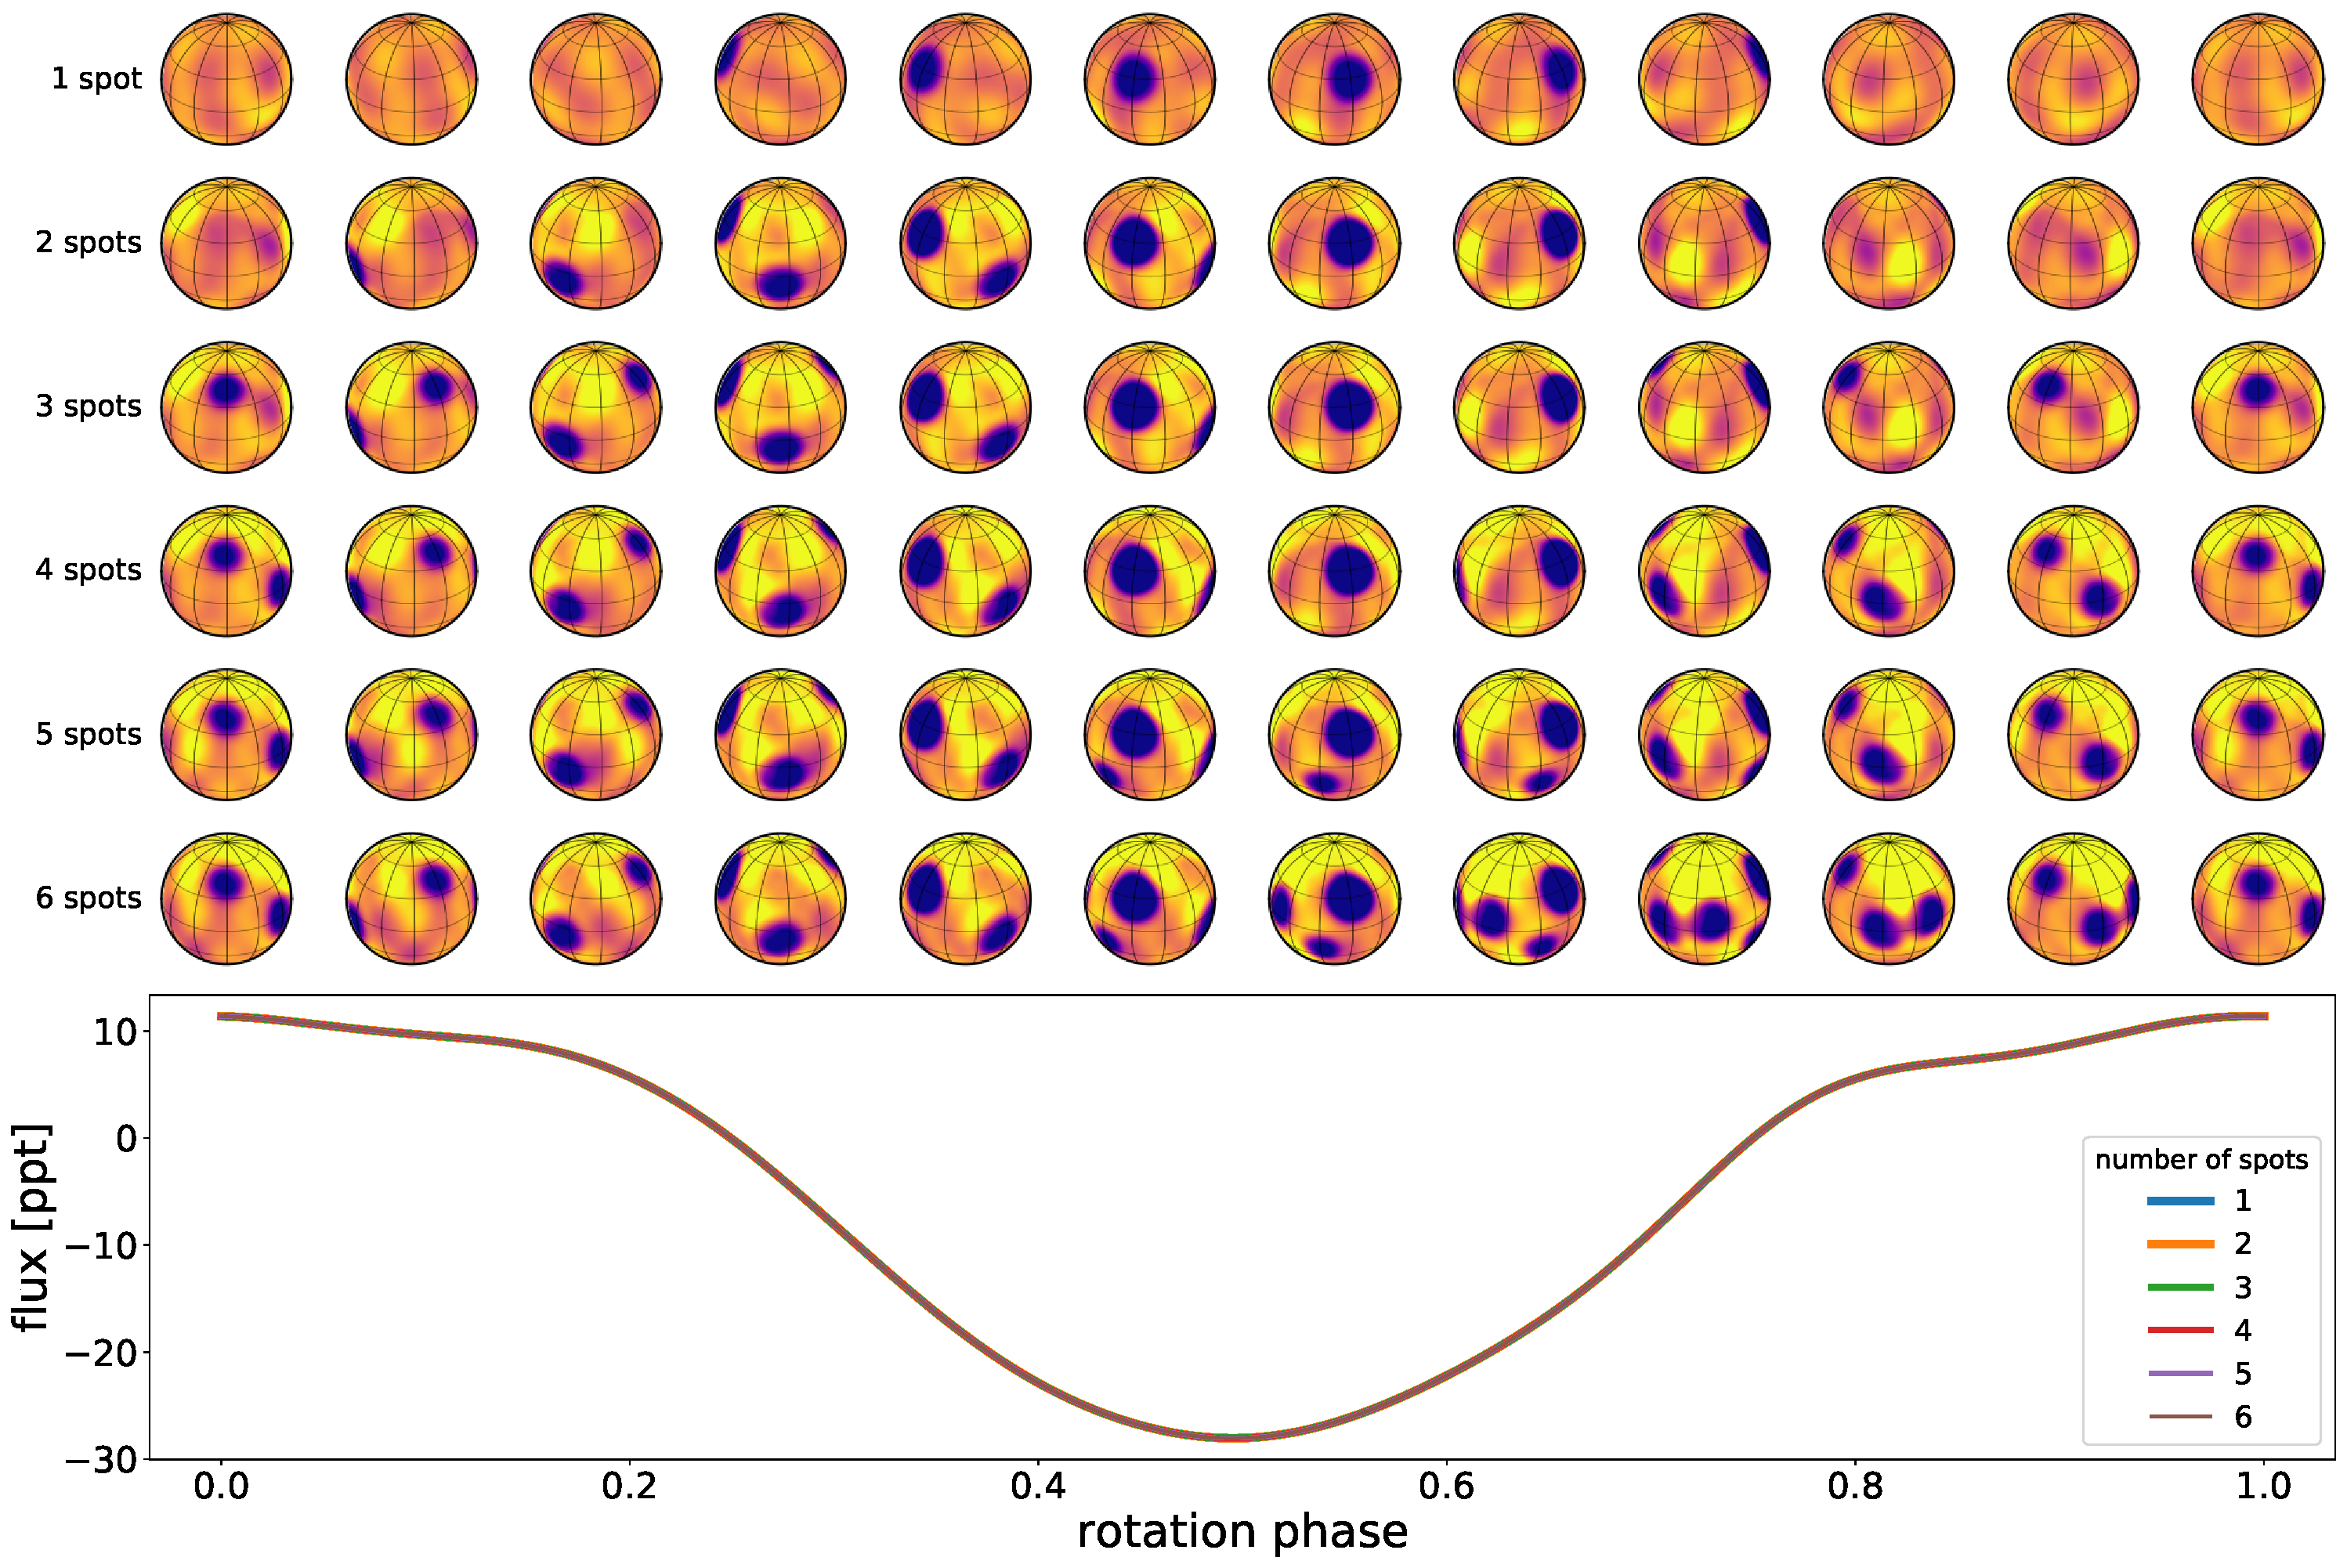
\includegraphics[width=\linewidth]{figures/degeneracies.pdf}
        \oscaption{degeneracies}{%
            The fundamental limitations of the mapping problem. Each row
            corresponds to a stellar surface with a different number of
            dark spots seen at various phases at an inclination $I=60^\circ$;
            all images are shown on the same color scale.
            The bottom panel shows the light curves of each of these stars.
            All six light curves are indistinguishable from each other, even
            at infinite signal to noise. See text for details.
            \label{fig:degeneracies}
        }
    \end{centering}
\end{figure}

While the stellar surfaces are all distinct, containing between one (top)
and six (bottom) large dark spots,
\textbf{their rotational light curves are identical}
(lower panel). This is true even at infinite signal to
noise: the mapping from a stellar surface
to its rotational light curve is so degenerate that there exist an infinite number of solutions
to the inverse problem. This fact has been pointed out recently in different contexts
\citep[e.g.,][]{Cowan2013,Luger2019,Basri2020}, but it dates back at least to
\citet{Russell1906}, who demonstrated it by expanding the surface
intensity of a celestial body in terms of spherical harmonics
(see \S\ref{sec:main} and Figure~\ref{fig:ylms}). \citet{Russell1906} showed
that many of the modes comprising the intensity profile of a spherical
object are in the \emph{null space}, the set of surface features that have identically
zero effect on the light curve. In fact,
the \emph{vast majority} of the modes are in the null space for rotational
light curves of stars (\S\ref{sec:nullspace}). This is what allows us to construct pathological
scenarios like that shown in Figure~\ref{fig:degeneracies}, where the light curve
could be explained by any number of spots atop a heterogeneous bright background.

Stellar mapping studies tackle these degeneracies in different ways, but
it usually comes down to a choice of prior: when the data is not
sufficiently informative, prior assumptions are needed to discriminate
between competing solutions. In discrete spot models like the ones
discussed above, the degeneracy-breaking prior is (typically) the assumption that the
spots must be circular, have uniform contrast, and sit atop an otherwise
uniform photosphere. In gridded stellar surface models, it is common to
assume a regularization prior such as the maximum entropy penalty
\citep[e.g.,][]{Vogt1987}, which typically favors solutions with the fewest
number of dark pixels (usually referred to as the ``simplest'' solution).

While these assumptions may be approximately valid in some cases, it is
important to bear in mind that because of the light curve degeneracies discussed above,
\textbf{most of the information about the stellar surface usually comes from the prior},
so it is very important to get the
prior right. In general, sunspots are not circular and do not have uniform
contrast throughout; nor do spots always arrange themselves in the highest
entropy configuration. The amount of bias introduced by these assumptions
will in general vary, but in principle it could be quite significant.

% Add to this photometric noise, the generally unknown stellar inclination,
% the poorly constrained limb darkening parameters, and you get ... a mess.

Fortunately, although individual light curves are not very constraining,
we have \emph{a lot of them} thanks to missions like \emph{Kepler} and \emph{TESS}.
In this paper, we will thoroughly explore the power of ensemble analyses
in breaking the degeneracies inherent to the light curve mapping problem.
By jointly analyzing the light curves of many stars, we will show that it
is often possible to uniquely constrain statistical properties about their
surfaces. This idea was recently explored to some extent
in \citet{Morris2020}, who used ensemble analyses to derive constraints on
spot coverage areas as a function of stellar age (see \S\ref{sec:other-work}).

\bibliography{bib}

\end{document}
